\documentclass[tikz,border=6pt]{standalone}
\usetikzlibrary{arrows.meta,calc}

\begin{document}
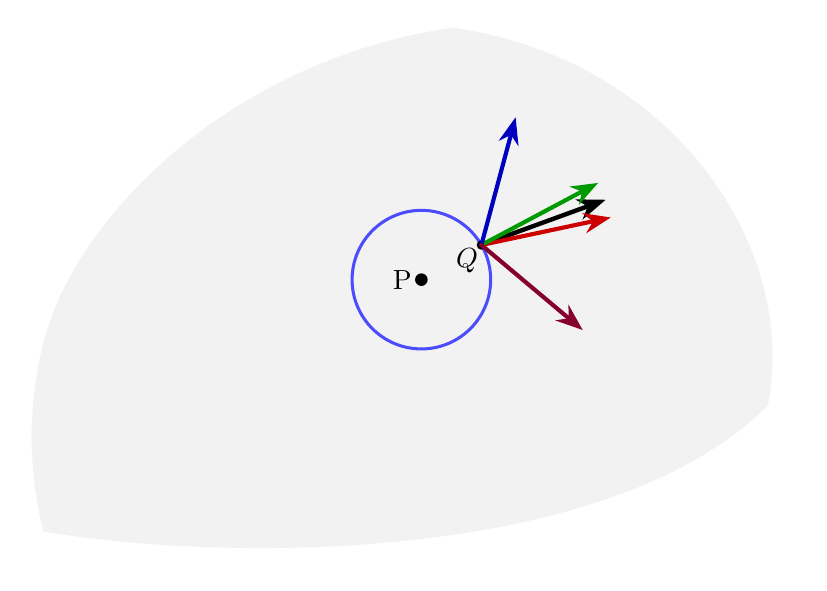
\begin{tikzpicture}[scale=4, line cap=round, line join=round]

% --- Surface patch (smooth convex patch) ---
\fill[gray!10] (-1.2,-0.8) .. controls (-0.6,-0.9) and (0.6,-0.9) .. (1.1,-0.4)
                 .. controls (1.2,0.1) and (0.8,0.7) .. (0.1,0.8)
                 .. controls (-0.6,0.7) and (-1.1,0.2) .. (-1.2,-0.2)
                 .. controls (-1.25,-0.4) and (-1.25,-0.6) .. cycle;

% --- Base point P (center of loop) ---
\coordinate (P) at (0,0);
\fill[black] (P) circle (0.02) node[left] {P};

% --- Small loop centered at P ---
\def\looprad{0.22}
\draw[line width=1.1pt,blue!70] ($(P)+(\looprad,0)$) arc[start angle=0,end angle=360,radius=\looprad];

% --- Choose a point Q on the loop (move vectors here) ---
\def\phi{30} % degrees on the loop where you want to anchor the vectors
\coordinate (Q) at ($(P)+(\phi:\looprad)$);
\fill[black] (Q) circle (0.015) node[inner sep=1pt,below left] {$Q$};

% Optional: spoke from P to Q for reference
%\draw[dashed,orange!80,very thick] (P)--(Q);

% --- One coordinate curve that is a geodesic (black) passing through P (optional) ---
% \draw[line width=0.7pt,black]
%   (-1.0,-0.15) .. controls (-0.5,-0.05) and (-0.2,0.02) .. (P)
%   .. controls (0.35,0.06) and (0.7,0.10) .. (1.05,0.15);

% --- Common vector parameters (unchanged directions/lengths) ---
\def\ang{20}     % initial direction in degrees
\def\Len{0.42}   % uniform length for all vectors

% --- Initial vector v anchored at Q (was at P) ---
\draw[->,line width=1.6pt,black,>=Stealth] (Q) -- ++(\ang:\Len);

% --- Candidate transported vectors anchored at Q (all tails exactly at Q) ---
% Red: small clockwise rotation (correct small holonomy for K > 0)
\draw[->,line width=1.5pt,red!80!black,>=Stealth] (Q) -- ++({\ang-8}:\Len);

% Green: small counterclockwise rotation (distractor)
\draw[->,line width=1.5pt,green!60!black,>=Stealth] (Q) -- ++({\ang+8}:\Len);

% Blue: large counterclockwise rotation (distractor)
\draw[->,line width=1.5pt,blue!75!black,>=Stealth] (Q) -- ++({\ang+55}:\Len);

% Purple: large clockwise rotation (distractor)
\draw[->,line width=1.5pt,purple!70!black,>=Stealth] (Q) -- ++({\ang-60}:\Len);

\end{tikzpicture}
\end{document}